\usetikzlibrary{patterns, positioning, arrows.meta}

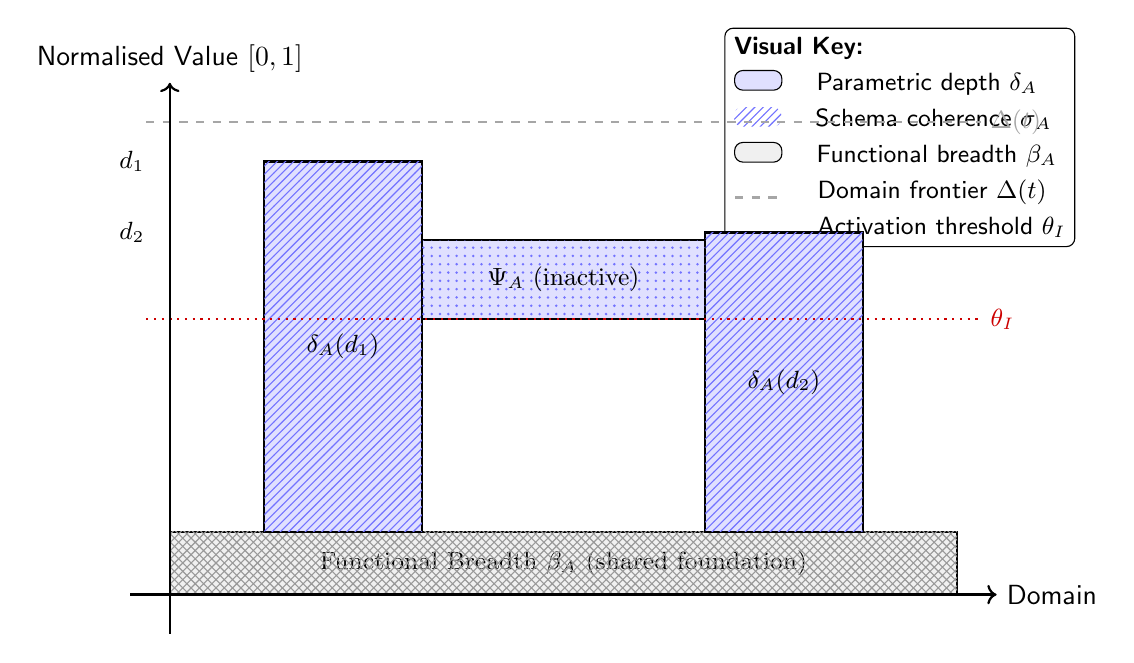
\begin{tikzpicture}[font=\sffamily]

    % Define colors (Okabe-Ito compatible for grayscale)
    \colorlet{depthcolor}{blue!12}
    \colorlet{breadthcolor}{gray!12}
    \colorlet{schemacolor}{blue!55}
    \colorlet{frontiercolor}{gray!70}

    % ===== LEGEND (top right) =====
    \node[draw=black, rounded corners=3pt, fill=white, align=left, font=\small\sffamily, anchor=north east] at (11.5, 7.2) {
        \textbf{Visual Key:}\\[2pt]
        \tikz\fill[fill=depthcolor, draw=black] (0,0) rectangle (0.6,0.25); \quad Parametric depth $\delta_A$\\[2pt]
        \tikz\fill[pattern=north east lines, pattern color=schemacolor] (0,0) rectangle (0.6,0.25); \quad Schema coherence $\sigma_A$\\[2pt]
        \tikz\fill[fill=breadthcolor, draw=black] (0,0) rectangle (0.6,0.25); \quad Functional breadth $\beta_A$\\[2pt]
        \tikz\draw[dashed, thick, frontiercolor] (0,0.12) -- (0.6,0.12); \quad Domain frontier $\Delta(t)$\\[2pt]
        \tikz\draw[dotted, thick, red!80!black] (0,0.12) -- (0.6,0.12); \quad Activation threshold $\theta_I$
    };

    % 1. The Breadth Base (crosshatch pattern for grayscale)
    \filldraw[fill=breadthcolor, draw=black, thick] (0,0) rectangle (10, 0.8) node[midway, font=\small] {Functional Breadth $\beta_A$ (shared foundation)};
    \fill[pattern=crosshatch, pattern color=black!40] (0,0) rectangle (10, 0.8);

    % 2. The Depth Pillars (with Schema Texture)
    % Domain 1
    \filldraw[fill=depthcolor, draw=black, thick] (1.2, 0.8) rectangle (3.2, 5.5);
    \fill[pattern=north east lines, pattern color=schemacolor] (1.2, 0.8) rectangle (3.2, 5.5);
    \node[font=\small] at (2.2, 3.15) {$\delta_A(d_1)$};

    % Domain 2
    \filldraw[fill=depthcolor, draw=black, thick] (6.8, 0.8) rectangle (8.8, 4.6);
    \fill[pattern=north east lines, pattern color=schemacolor] (6.8, 0.8) rectangle (8.8, 4.6);
    \node[font=\small] at (7.8, 2.7) {$\delta_A(d_2)$};

    % 3. The Intersection Bridge (dots pattern for grayscale distinction)
    \filldraw[fill=depthcolor, draw=black, thick] (3.2, 3.5) rectangle (6.8, 4.5);
    \fill[pattern=dots, pattern color=schemacolor] (3.2, 3.5) rectangle (6.8, 4.5);
    \node[font=\small] at (5, 4) {$\Psi_A$ (inactive)};

    % 4. Thresholds and Frontiers
    \draw[dashed, thick, frontiercolor] (-0.3, 6.0) -- (10.3, 6.0);
    \node[anchor=west, font=\small, text=frontiercolor] at (10.3, 6.0) {$\Delta(t)$};

    \draw[dotted, thick, red!80!black] (-0.3, 3.5) -- (10.3, 3.5);
    \node[anchor=west, font=\small, text=red!80!black] at (10.3, 3.5) {$\theta_I$};

    % 5. Axis labels
    \draw[->, thick] (0, -0.5) -- (0, 6.5) node[above] {Normalised Value $[0, 1]$};
    \draw[->, thick] (-0.5, 0) -- (10.5, 0) node[right] {Domain};
    \node[anchor=east, font=\small] at (-0.2, 5.5) {$d_1$};
    \node[anchor=east, font=\small] at (-0.2, 4.6) {$d_2$};

\end{tikzpicture}
